\documentclass[xelatex,ja=standard,jafont=noto]{bxjsarticle}
\usepackage[utf8]{inputenc}

\date{May 2020}

\usepackage{natbib}
\usepackage{graphicx}
\usepackage{tikz}
\usepackage{circuitikz}
\usepackage{tabularx}
\usepackage{diagbox}



\begin{document}



	\begin{titlepage}
			\begin{center}
				
				{\Large 令和2年}
				
				\vspace{10truept}
				
				{\Large 機械工学実験1}
				
				\vspace*{140truept}
				
				{\Huge デジタル回路プリレポート} 
				
				\vspace{160truept}
				
				{\Large 指導教員}
				
				\vspace{10truept}
				
				{\Large yoshitaka adachi}
				
				\vspace{70truept}
				
				{\Large 芝浦工業大学}
				
				\vspace{10truept}
				
				{\Large 機械制御システム}
				
				\vspace{30truept}
				
				{\Large bq18026 関宇}      
				
			\end{center}
		\end{titlepage}








\section{課題1}
図 2 の回路について,vi(t) = u(t) = 0,vo(0) = 5 として横軸 t,縦軸 vo(t) のグラフを描け.
		
\begin{figure}[h!]
  \begin{center}
    \begin{circuitikz}
      \draw (0,0)
      to[V,v=$U_i$] (0,2)
      to[R=$R$] (2,2)
      to[C=$C$] (2,0) 
      to[short] (0,0);
    \end{circuitikz}
    \caption{RC circuit.}
  \end{center}
\end{figure}



\iffalse
ここでコメント
\fi





回路方程式からラプラス変換をを計算し、$  V_{0}(s) $について解けば次式になる
	\begin{equation}
		 V_{0}(s)=\frac{CR}{CRs+1}V_{i}(s)+\frac{CR}{CRs+1}e_{0}(0)
	\end{equation}
$  v_{i}(t) $=$  v(t) $=0より、
    \begin{equation}
		 V_{0}(s)=\frac{CR}{CRs+1}e_{0}(0)
	\end{equation}
ラプラス逆変換し、$ e_{0}(0) $=5を代入すると
    \begin{equation}
		 v_{0}(t)=5	e^{-\frac{t}{T}} \hspace{2mm}(T=CR)
	\end{equation}

C=1pF,R=1$ \Omega $を$  v_{0}(t) $に代入してグラフを書く。

\begin{figure}[h!]
    \centering
    \includegraphics[scale=0.4]{untitled.jpg}
    \caption{$  v_{0}(t) $のグラフ}
\end{figure}






\iffalse
ここでコメント
\fi



\newpage






\section{課題2}

\begin{equation}
		X=\bar{A}\bar{B}\bar{C}D+\bar{A}\bar{B}CD+\bar{A}BCD+A\bar{B}\bar{C}D
\end{equation}

をKarnaugh map methodを用いてを用いて簡素化する.\\
4変量のカルノー図について表のようになる

\begin{table}[!htbp]
\centering
\begin{tabular}{ |c|c|c|c|c| } 
 \hline
 \diagbox[]{AB}{CD} & 00 & 01 & 11 & 10 \\ 
 \hline
 00 & 1 & 2 & 4 & 3\\ 
 \hline
 01 & 5 & 6 & 8 & 7 \\ 
 \hline
 11 & 9 & 10 & 12 & 11 \\ 
 \hline
 10 & 13 & 14 & 16 & 15 \\ 
 \hline
\end{tabular}
\caption{カルノー図.}
\end{table}

関係式より
\begin{equation}
		X=(A,B,C,D)=\Sigma m(2,4,6,8,14)
\end{equation}

表に表示すると

\begin{table}[!htbp]
\centering
\begin{tabular}{ |c|c|c|c|c| } 
 \hline
 \hline
 \diagbox[]{AB}{CD} & 00 & 01 & 11 & 10 \\ 
 \hline
 00 & 0 & 1 & 1 & 0\\ 
 \hline
 01 & 0 & 1 & 1 & 0 \\ 
 \hline
 11 & 0 & 0 & 0 & 0 \\ 
 \hline
 10 & 0 & 1 & 0 & 0 \\ 
 \hline
\end{tabular}
\caption{カルノー図.}
\end{table}
表の中で1の部分を分析すると

\begin{equation}
		X=\bar{A}D+\bar{B}\bar{C}D
\end{equation}




\iffalse
ここでコメント
\fi





\section{課題3}
図 8 において,AND ゲート(7408)の出力が OR ゲート(7432)の入力に接続されている.使
用するデジタル IC を,7408 は SN74HC08,7432 は SN74HC32 として,これらのデータシートを読んで下記の問いに答えよ.なお,デジタル IC の電源電圧(Vcc)を 4.5V とする.

\subsection{SN74HC32 の入力端子において,入力電圧を“H”と認識する最低入力電圧$  V_{IH} $ は何ボルトか? 入力電圧を“L”と認識する最大入力電圧 $  V_{IL} $ は何ボルトか?}

データシートより、SN74HC32の入力電圧を“H”と認識する最低入力電圧$  V_{IH} $ =3.15V.
入力電圧を“L”と認識する最大入力電圧 $  V_{IL} $ =1.35V

\subsection{SN74HC08 の出力端子において,“H”を出力する場合の最低出力電圧 VOH は何ボルトか?“L”を出力する場合の最大出力電圧 $  V_{OL} $  は何ボルトか?}

データシートより、“H”を出力する場合の最低出力電圧$  V_{OH} $=4.4V.
“L”を出力する場合の最大出力電圧 $  V_{OL} $ =0.1V

\subsection{図 8 において AND ゲート(SN74HC08)の出力を OR ゲート(SN74HC32)の入力に接続しても問題が無いという理由を説明せよ.}

OR ゲート(SN74HC32)に入力した電圧が認識できるため、必ず(0V-1.35V,Low signal),あるいは(3.15V-4.5V,High signal)にしなければいけない。SN74HC08の“H”を出力する場合の最低出力電圧$  V_{OH} $と “L”を出力する場合の最大出力電圧 $  V_{OL} $とともに認識できる範囲内なので、
接続しても問題がない。






\iffalse
ここでコメント
\fi







\section{課題4}
ハイスピード CMOS のインバータ(SN74HC04)とANDゲート(SN74HC08)を使って図 15
のような回路を組むことにする.インバータ(SN74HC04)のファンアウトを求めよ.

\begin{equation}
	\mbox{インバータ(SN74HC04)のファンアウト}=\frac{\mbox{負荷容量} C_{L}}{\mbox{入力容量} C_{IN}}
\end{equation}
各物件のデータシートより
\begin{equation}
	\mbox{インバータ(SN74HC04)のファンアウト}=\frac{50pF}{10pF}=5
\end{equation}





\iffalse
ここでコメント
\fi






\section{課題5}
\subsection{インクリメンタルエンコーダにおけるA相,B相の役割と,正転・逆転の判定方法を述べよ.}
A相、B相の役割はモータの回転方向を判別するである。正転の時、A相に対してB相が$  \frac{\pi}{4} $遅れて出力されている.逆転の時、$  \frac{\pi}{4} $進んで出力されている.
\subsection{インクリメンタルエンコーダにおけるZ相の役割を考察せよ.}
Z相の役割はモータの回転数を数えることである.一回転しZ相の光が一回穴に通過し、パルス信号が一回出ているので、回転数がパルス数で分かる。
\subsection{DC モータが3000rpmで回転したとき,インクリメンタルエンコーダのA相の周波数と周期を求めよ.}
実験で使われているインクリメンタルエンコーダは一回転100パルスが生じっている。さらにモータが3000rpmで回転した上て、一秒あたり50回転である。\\
よって、A相の周波数は

\begin{equation}
	50\times 100=5K{Hz}
\end{equation}
A相の周期は
\begin{equation}
	\frac{1}{5000}=0.0002{s}
\end{equation}





\iffalse
ここでコメント
\fi







\section{課題6}
\subsection{SN74HC04が「H」レベルVOHを出力するとき,最も高い電圧(TYP)と最も低い電圧(MIN)は何 V か?}
データシートより,SN74HC04が「H」レベルVOHを出力するとき,最も高い電圧(TYP)は4.499V.最も低い電圧(MIN)は4.4V.

\subsection{SN74HC04が「L」レベルVOLを出力するとき,最も低い電圧(TYP)と最も高い電圧(MAX)は何 V か?}
データシートより,SN74HC04が「L」レベルVOLを出力するとき,最も低い電圧(TYP)は0.001V,最も高い電圧(MAX)は0.1V.

\subsection{SN74HC00が入力信号を「L」と判断する最大電圧(VIL)は何Vか?また入力信号を「H」と判断する最低電圧(VIH)は何 V か?}

データシートより,SN74HC00が入力信号を「L」と判断する最大電圧(VIL)は1.35V,
「H」と判断する最低電圧(VIH)は3.15V.





\iffalse
ここでコメント
\fi





\newpage

\section{課題7}
DC モータが 3000rpm で回転しているときのタイミングチャートを描け.ただし描くポイ
ントは,回路図左上の 7404(インバータ)の入力(端子番号1)と出力(端子番号2),7400
(NAND ゲート)の入力(端子番号1,2)と出力(端子番号3)とする.図 30 を参考にすること.\\

まず、7404の入力がA相そのままで、周期は0.0002{s}=200usである。

\begin{figure}[h!]
\begin{center}
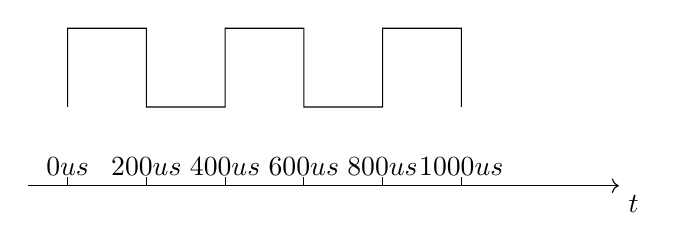
\begin{tikzpicture}[scale=1]

\coordinate (P) at (0.5, 0);
\coordinate (A) at (1, 0);
\coordinate (B) at (2, 0);
\coordinate (C) at (3, 0);
\coordinate (D) at (4, 0);
\coordinate (E) at (5, 0);
\coordinate (F) at (6, 0);
\coordinate (Q) at (8, 0);

\draw (A) node[above] {$0us$} -- ++(0, 3pt) ;
\draw (B) node[above] {$200us$} -- ++(0, 3pt);
\draw (C) node[above] {$400us$} -- ++(0, 3pt) ;
\draw (D) node[above] {$600us$} -- ++(0, 3pt) ;
\draw (E) node[above] {$800us$} -- ++(0, 3pt) ;
\draw (F) node[above] {$1000us$} -- ++(0, 3pt) ;

\draw[->] (P)--(Q) node [below right]{$t$};

\draw (1,1)
to[short] (1,2)
to[short] (2,2)
to[short] (2,1)
to[short] (3,1)
to[short] (3,2)
to[short] (4,2)
to[short] (4,1)
to[short] (5,1)
to[short] (5,2)
to[short] (6,2)
to[short] (6,1); 

\end{tikzpicture}
\caption{7404\ 01 \ timing chart}
\end{center}
\end{figure}

入力信号がNOTゲートに通過し、逆位相になる。


\begin{figure}[h!]
\begin{center}
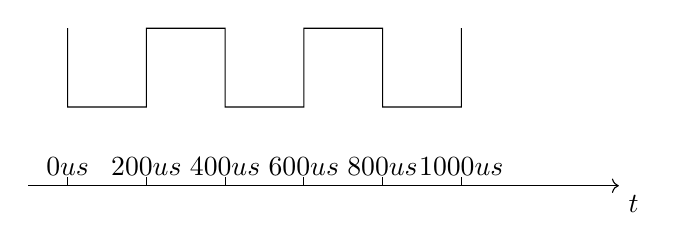
\begin{tikzpicture}[scale=1]

\coordinate (P) at (0.5, 0);
\coordinate (A) at (1, 0);
\coordinate (B) at (2, 0);
\coordinate (C) at (3, 0);
\coordinate (D) at (4, 0);
\coordinate (E) at (5, 0);
\coordinate (F) at (6, 0);
\coordinate (Q) at (8, 0);

\draw (A) node[above] {$0us$} -- ++(0, 3pt) ;
\draw (B) node[above] {$200us$} -- ++(0, 3pt);
\draw (C) node[above] {$400us$} -- ++(0, 3pt) ;
\draw (D) node[above] {$600us$} -- ++(0, 3pt) ;
\draw (E) node[above] {$800us$} -- ++(0, 3pt) ;
\draw (F) node[above] {$1000us$} -- ++(0, 3pt) ;

\draw[->] (P)--(Q) node [below right]{$t$};

\draw (1,2)
to[short] (1,1)
to[short] (2,1)
to[short] (2,2)
to[short] (3,2)
to[short] (3,1)
to[short] (4,1)
to[short] (4,2)
to[short] (5,2)
to[short] (5,1)
to[short] (6,1)
to[short] (6,2); 

\end{tikzpicture}
\caption{7404\ 02 \ timing chart}
\end{center}
\end{figure}

7400の入力の一つはA相そのまま、もう一つはRC回路に通過したので、課題1の結論をそこで利用する。

\begin{figure}[h!]
\begin{center}
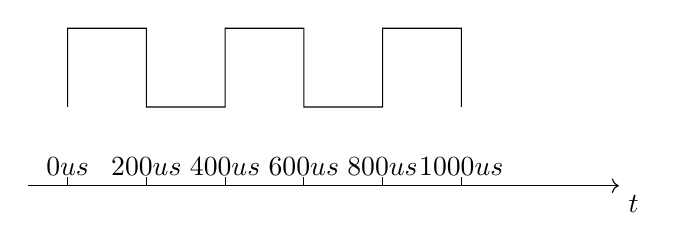
\begin{tikzpicture}[scale=1]

\coordinate (P) at (0.5, 0);
\coordinate (A) at (1, 0);
\coordinate (B) at (2, 0);
\coordinate (C) at (3, 0);
\coordinate (D) at (4, 0);
\coordinate (E) at (5, 0);
\coordinate (F) at (6, 0);
\coordinate (Q) at (8, 0);

\draw (A) node[above] {$0us$} -- ++(0, 3pt) ;
\draw (B) node[above] {$200us$} -- ++(0, 3pt);
\draw (C) node[above] {$400us$} -- ++(0, 3pt) ;
\draw (D) node[above] {$600us$} -- ++(0, 3pt) ;
\draw (E) node[above] {$800us$} -- ++(0, 3pt) ;
\draw (F) node[above] {$1000us$} -- ++(0, 3pt) ;

\draw[->] (P)--(Q) node [below right]{$t$};

\draw (1,1)
to[short] (1,2)
to[short] (2,2)
to[short] (2,1)
to[short] (3,1)
to[short] (3,2)
to[short] (4,2)
to[short] (4,1)
to[short] (5,1)
to[short] (5,2)
to[short] (6,2)
to[short] (6,1); 

\end{tikzpicture}
\caption{7400\ 01 \ timing chart}
\end{center}
\end{figure}



\begin{figure}[h!]
\begin{center}
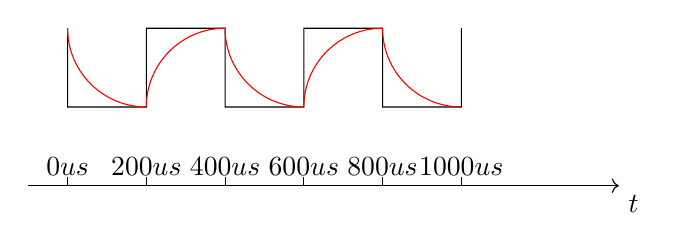
\begin{tikzpicture}[scale=1]

\coordinate (P) at (0.5, 0);
\coordinate (A) at (1, 0);
\coordinate (B) at (2, 0);
\coordinate (C) at (3, 0);
\coordinate (D) at (4, 0);
\coordinate (E) at (5, 0);
\coordinate (F) at (6, 0);
\coordinate (Q) at (8, 0);

\draw (A) node[above] {$0us$} -- ++(0, 3pt) ;
\draw (B) node[above] {$200us$} -- ++(0, 3pt);
\draw (C) node[above] {$400us$} -- ++(0, 3pt) ;
\draw (D) node[above] {$600us$} -- ++(0, 3pt) ;
\draw (E) node[above] {$800us$} -- ++(0, 3pt) ;
\draw (F) node[above] {$1000us$} -- ++(0, 3pt) ;

\draw[->] (P)--(Q) node [below right]{$t$};

\draw (1,2)
to[short] (1,1)
to[short] (2,1)
to[short] (2,2)
to[short] (3,2)
to[short] (3,1)
to[short] (4,1)
to[short] (4,2)
to[short] (5,2)
to[short] (5,1)
to[short] (6,1)
to[short] (6,2); 

\draw[red](2,1) arc (270:180:1);
\draw[red](3,2) arc (90:180:1);
\draw[red](4,1) arc (270:180:1);
\draw[red](5,2) arc (90:180:1);
\draw[red](6,1) arc (270:180:1);

\end{tikzpicture}
\caption{7400\ 02 \ timing chart}
\end{center}
\end{figure}
\newpage

NANDゲートの出力はNANDの真理値表を参考すると、全ての入力が0の時に出力が0、その他の場合は全ての出力が1.赤い線で出力を表示すると図のようになる。

\begin{figure}[h!]
\begin{center}
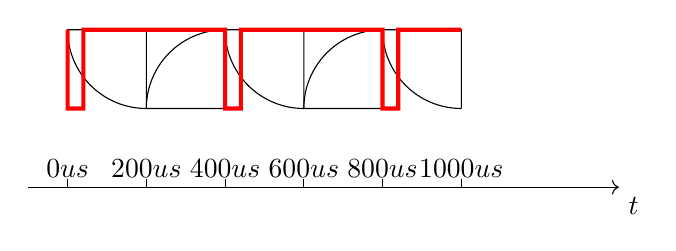
\begin{tikzpicture}[scale=1]

\coordinate (P) at (0.5, 0);
\coordinate (A) at (1, 0);
\coordinate (B) at (2, 0);
\coordinate (C) at (3, 0);
\coordinate (D) at (4, 0);
\coordinate (E) at (5, 0);
\coordinate (F) at (6, 0);
\coordinate (Q) at (8, 0);

\draw (A) node[above] {$0us$} -- ++(0, 3pt) ;
\draw (B) node[above] {$200us$} -- ++(0, 3pt);
\draw (C) node[above] {$400us$} -- ++(0, 3pt) ;
\draw (D) node[above] {$600us$} -- ++(0, 3pt) ;
\draw (E) node[above] {$800us$} -- ++(0, 3pt) ;
\draw (F) node[above] {$1000us$} -- ++(0, 3pt) ;

\draw[->] (P)--(Q) node [below right]{$t$};

\draw (1,1)
to[short] (1,2)
to[short] (2,2)
to[short] (2,1)
to[short] (3,1)
to[short] (3,2)
to[short] (4,2)
to[short] (4,1)
to[short] (5,1)
to[short] (5,2)
to[short] (6,2)
to[short] (6,1); 
\draw(2,1) arc (270:180:1);
\draw(3,2) arc (90:180:1);
\draw(4,1) arc (270:180:1);
\draw(5,2) arc (90:180:1);
\draw(6,1) arc (270:180:1);

\draw[red,line width=1.5] (1,2)
to[short] (1,1)
to[short](1.2,1)
to[short](1.2,2)
to[short](3,2)
to[short](3,1)
to[short](3.2,1)
to[short](3.2,2)
to[short](5,2)
to[short](5,1)
to[short](5.2,1)
to[short](5.2,2)
to[short](6,2);

\end{tikzpicture}
\caption{7400\ 03 \ timing chart}
\end{center}
\end{figure}







\iffalse
ここでコメント
\fi








\section{課題8}
\subsection{実験用の回路ではロータリーエンコーダが出力するA相とB 相の位相差から回転方向を弁
別する.図 31 のタイミングチャートを完成させなさい.}

課題5を参考し、正転の時にB相が遅れて出力されている。

\begin{figure}[h!]
\begin{center}
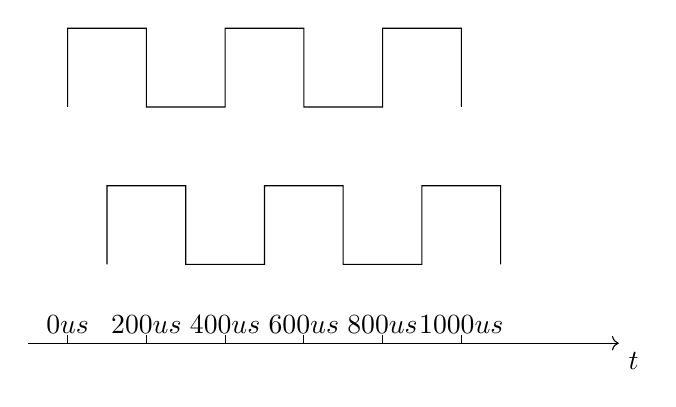
\begin{tikzpicture}[scale=1]

\coordinate (P) at (0.5, 0);
\coordinate (A) at (1, 0);
\coordinate (B) at (2, 0);
\coordinate (C) at (3, 0);
\coordinate (D) at (4, 0);
\coordinate (E) at (5, 0);
\coordinate (F) at (6, 0);
\coordinate (Q) at (8, 0);

\draw (A) node[above] {$0us$} -- ++(0, 3pt) ;
\draw (B) node[above] {$200us$} -- ++(0, 3pt);
\draw (C) node[above] {$400us$} -- ++(0, 3pt) ;
\draw (D) node[above] {$600us$} -- ++(0, 3pt) ;
\draw (E) node[above] {$800us$} -- ++(0, 3pt) ;
\draw (F) node[above] {$1000us$} -- ++(0, 3pt) ;

\draw[->] (P)--(Q) node [below right]{$t$};

\draw (1,3)
to[short] (1,4)
to[short] (2,4)
to[short] (2,3)
to[short] (3,3)
to[short] (3,4)
to[short] (4,4)
to[short] (4,3)
to[short] (5,3)
to[short] (5,4)
to[short] (6,4)
to[short] (6,3); 

\draw (1.5,1)
to[short] (1.5,2)
to[short] (2.5,2)
to[short] (2.5,1)
to[short] (3.5,1)
to[short] (3.5,2)
to[short] (4.5,2)
to[short] (4.5,1)
to[short] (5.5,1)
to[short] (5.5,2)
to[short] (6.5,2)
to[short] (6.5,1);

\end{tikzpicture}
\caption{正転の時のA相B相}
\end{center}
\end{figure}

7400の3番の信号がB相の信号とともにLの時ORゲートの出力がLになって、そこでパルス信号が生じる。赤線に表示する。

\begin{figure}[h!]
\begin{center}
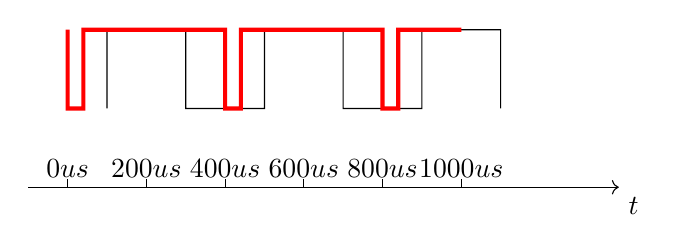
\begin{tikzpicture}[scale=1]

\coordinate (P) at (0.5, 0);
\coordinate (A) at (1, 0);
\coordinate (B) at (2, 0);
\coordinate (C) at (3, 0);
\coordinate (D) at (4, 0);
\coordinate (E) at (5, 0);
\coordinate (F) at (6, 0);
\coordinate (Q) at (8, 0);

\draw (A) node[above] {$0us$} -- ++(0, 3pt) ;
\draw (B) node[above] {$200us$} -- ++(0, 3pt);
\draw (C) node[above] {$400us$} -- ++(0, 3pt) ;
\draw (D) node[above] {$600us$} -- ++(0, 3pt) ;
\draw (E) node[above] {$800us$} -- ++(0, 3pt) ;
\draw (F) node[above] {$1000us$} -- ++(0, 3pt) ;

\draw[->] (P)--(Q) node [below right]{$t$};

\draw (1.5,1)
to[short] (1.5,2)
to[short] (2.5,2)
to[short] (2.5,1)
to[short] (3.5,1)
to[short] (3.5,2)
to[short] (4.5,2)
to[short] (4.5,1)
to[short] (5.5,1)
to[short] (5.5,2)
to[short] (6.5,2)
to[short] (6.5,1);

\draw[red,line width=1.5] (1,2)
to[short] (1,1)
to[short](1.2,1)
to[short](1.2,2)
to[short](3,2)
to[short](3,1)
to[short](3.2,1)
to[short](3.2,2)
to[short](5,2)
to[short](5,1)
to[short](5.2,1)
to[short](5.2,2)
to[short](6,2);


\end{tikzpicture}
\caption{7432\ 03 \ timing chart}
\end{center}
\end{figure}

\newpage
この時7432 6番の信号がパルスが生じない。


\begin{figure}[h!]
\begin{center}
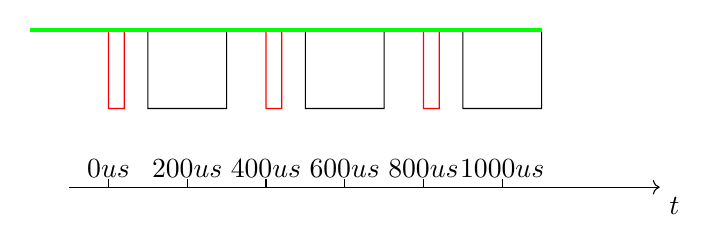
\begin{tikzpicture}[scale=1]

\coordinate (P) at (0.5, 0);
\coordinate (A) at (1, 0);
\coordinate (B) at (2, 0);
\coordinate (C) at (3, 0);
\coordinate (D) at (4, 0);
\coordinate (E) at (5, 0);
\coordinate (F) at (6, 0);
\coordinate (Q) at (8, 0);

\draw (A) node[above] {$0us$} -- ++(0, 3pt) ;
\draw (B) node[above] {$200us$} -- ++(0, 3pt);
\draw (C) node[above] {$400us$} -- ++(0, 3pt) ;
\draw (D) node[above] {$600us$} -- ++(0, 3pt) ;
\draw (E) node[above] {$800us$} -- ++(0, 3pt) ;
\draw (F) node[above] {$1000us$} -- ++(0, 3pt) ;

\draw[->] (P)--(Q) node [below right]{$t$};

\draw (1.5,2)
to[short] (1.5,1)
to[short] (2.5,1)
to[short] (2.5,2)
to[short] (3.5,2)
to[short] (3.5,1)
to[short] (4.5,1)
to[short] (4.5,2)
to[short] (5.5,2)
to[short] (5.5,1)
to[short] (6.5,1)
to[short] (6.5,2);

\draw[red] (1,2)
to[short] (1,1)
to[short](1.2,1)
to[short](1.2,2)
to[short](3,2)
to[short](3,1)
to[short](3.2,1)
to[short](3.2,2)
to[short](5,2)
to[short](5,1)
to[short](5.2,1)
to[short](5.2,2)
to[short](6,2);

\draw[green,line width=1.5](0,2)
to[short] (6.5,2);


\end{tikzpicture}
\caption{7432 \ 06 \ timing chart}
\end{center}
\end{figure}

逆に、逆転の時B相が進んで出力されている。

\begin{figure}[h!]
\begin{center}
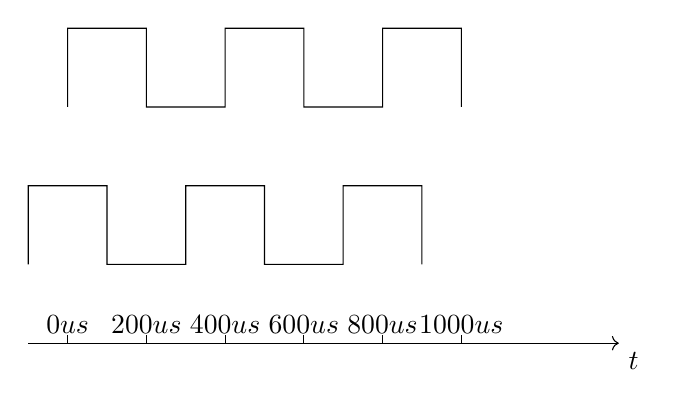
\begin{tikzpicture}[scale=1]

\coordinate (P) at (0.5, 0);
\coordinate (A) at (1, 0);
\coordinate (B) at (2, 0);
\coordinate (C) at (3, 0);
\coordinate (D) at (4, 0);
\coordinate (E) at (5, 0);
\coordinate (F) at (6, 0);
\coordinate (Q) at (8, 0);

\draw (A) node[above] {$0us$} -- ++(0, 3pt) ;
\draw (B) node[above] {$200us$} -- ++(0, 3pt);
\draw (C) node[above] {$400us$} -- ++(0, 3pt) ;
\draw (D) node[above] {$600us$} -- ++(0, 3pt) ;
\draw (E) node[above] {$800us$} -- ++(0, 3pt) ;
\draw (F) node[above] {$1000us$} -- ++(0, 3pt) ;

\draw[->] (P)--(Q) node [below right]{$t$};

\draw (0.5,1)
to[short] (0.5,2)
to[short] (1.5,2)
to[short] (1.5,1)
to[short] (2.5,1)
to[short] (2.5,2)
to[short] (3.5,2)
to[short] (3.5,1)
to[short] (4.5,1)
to[short] (4.5,2)
to[short] (5.5,2)
to[short] (5.5,1); 

\draw (1,3)
to[short] (1,4)
to[short] (2,4)
to[short] (2,3)
to[short] (3,3)
to[short] (3,4)
to[short] (4,4)
to[short] (4,3)
to[short] (5,3)
to[short] (5,4)
to[short] (6,4)
to[short] (6,3);


\end{tikzpicture}
\caption{逆転の時のA相B相}
\end{center}
\end{figure}


この時7432 3番の信号がパルスが生じない。


\begin{figure}[h!]
\begin{center}
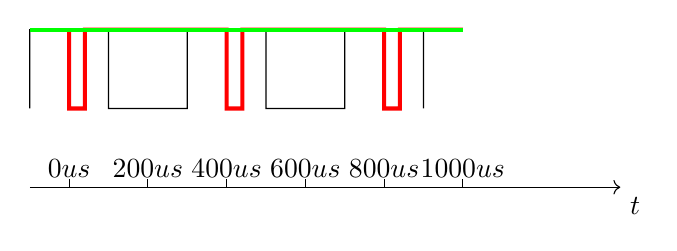
\begin{tikzpicture}[scale=1]

\coordinate (P) at (0.5, 0);
\coordinate (A) at (1, 0);
\coordinate (B) at (2, 0);
\coordinate (C) at (3, 0);
\coordinate (D) at (4, 0);
\coordinate (E) at (5, 0);
\coordinate (F) at (6, 0);
\coordinate (Q) at (8, 0);

\draw (A) node[above] {$0us$} -- ++(0, 3pt) ;
\draw (B) node[above] {$200us$} -- ++(0, 3pt);
\draw (C) node[above] {$400us$} -- ++(0, 3pt) ;
\draw (D) node[above] {$600us$} -- ++(0, 3pt) ;
\draw (E) node[above] {$800us$} -- ++(0, 3pt) ;
\draw (F) node[above] {$1000us$} -- ++(0, 3pt) ;

\draw[->] (P)--(Q) node [below right]{$t$};

\draw (0.5,1)
to[short] (0.5,2)
to[short] (1.5,2)
to[short] (1.5,1)
to[short] (2.5,1)
to[short] (2.5,2)
to[short] (3.5,2)
to[short] (3.5,1)
to[short] (4.5,1)
to[short] (4.5,2)
to[short] (5.5,2)
to[short] (5.5,1); 


\draw[red,line width=1.5] (1,2)
to[short] (1,1)
to[short](1.2,1)
to[short](1.2,2)
to[short](3,2)
to[short](3,1)
to[short](3.2,1)
to[short](3.2,2)
to[short](5,2)
to[short](5,1)
to[short](5.2,1)
to[short](5.2,2)
to[short](6,2);

\draw[green,line width=1.5] (0.5,2)
to[short] (6,2);


\end{tikzpicture}
\caption{7432\ 03 \ timing chart}
\end{center}
\end{figure}


7404 4番と7400 3番の信号がともにLの時7432 6番もLに出力されるので、パルス信号が生じる。


\begin{figure}[h!]
\begin{center}
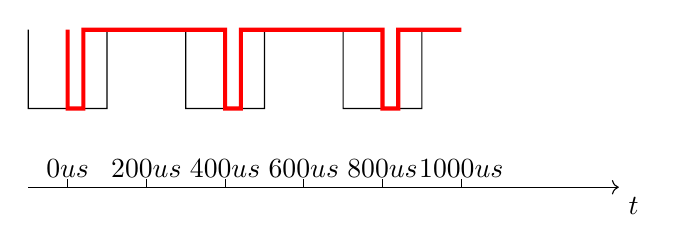
\begin{tikzpicture}[scale=1]

\coordinate (P) at (0.5, 0);
\coordinate (A) at (1, 0);
\coordinate (B) at (2, 0);
\coordinate (C) at (3, 0);
\coordinate (D) at (4, 0);
\coordinate (E) at (5, 0);
\coordinate (F) at (6, 0);
\coordinate (Q) at (8, 0);

\draw (A) node[above] {$0us$} -- ++(0, 3pt) ;
\draw (B) node[above] {$200us$} -- ++(0, 3pt);
\draw (C) node[above] {$400us$} -- ++(0, 3pt) ;
\draw (D) node[above] {$600us$} -- ++(0, 3pt) ;
\draw (E) node[above] {$800us$} -- ++(0, 3pt) ;
\draw (F) node[above] {$1000us$} -- ++(0, 3pt) ;

\draw[->] (P)--(Q) node [below right]{$t$};

\draw (0.5,2)
to[short] (0.5,1)
to[short] (1.5,1)
to[short] (1.5,2)
to[short] (2.5,2)
to[short] (2.5,1)
to[short] (3.5,1)
to[short] (3.5,2)
to[short] (4.5,2)
to[short] (4.5,1)
to[short] (5.5,1)
to[short] (5.5,2 ); 


\draw[red,line width=1.5] (1,2)
to[short] (1,1)
to[short](1.2,1)
to[short](1.2,2)
to[short](3,2)
to[short](3,1)
to[short](3.2,1)
to[short](3.2,2)
to[short](5,2)
to[short](5,1)
to[short](5.2,1)
to[short](5.2,2)
to[short](6,2);


\end{tikzpicture}
\caption{7432\ 06 \ timing chart}
\end{center}
\end{figure}

\newpage
\subsection{ロータリーエンコーダが出力する A 相と B 相の出力パルスは方向弁別回路の後,カウン
ター IC である 74192 に入力される.図 32 のタイミングチャートを完成させよ.}

課題の図32を分析し、一回パルス信号が入力されるとそれぞれの状況を考える。\\

まずカウントアップにパルス信号が12回入力され、そしてカウントダウンに5回入力され、十進数の算式で表すと12-5=7である。つまり、二進数の値を0から9まで、桁上がりし、12になってからカウントダウンを開始、最終7になる。\\

よって、74192のタイミングチャートが完成できる。

\begin{figure}[!htbp]
    \centering
    \includegraphics[scale=0.5]{wavedrom (2).png}
    \caption{74192 \ timing chart}
\end{figure}


\subsection{74192 の TERMINAL COUNT UP(CARRY) と TERMINAL COUNT DOWN(BORROW)
の出力信号は,図 33 においてどのように利用されているか説明せよ.}


カウントアップからのパルス信号が9まで入力して、さらに入力されるとCARRYにパルス信号が生じて、したの74192がプラスいち桁上がりした。逆にカウントダウンのパルス信号が3,2,1,0までさらに入力されると、BORROWにパルス信号が出て、桁下がりを発生する。






\iffalse
ここでコメント
\fi






\section{課題9}
LED 単体を点灯させる回路を図 28 に示す.LED に過電流が流れると焼損が発生するので,こ
の回路では電流制限用の抵抗 R が付けられている.端子 A-B 間の電位差を 5V として,LED を点
灯させるために 5mA~10mA を LED に流すためには,抵抗 R はどれだけの値にすればよいか?
ただし,LED の順方向電圧降下 VF を 2.0V とし,抵抗の値は E24 系列から選ぶものとする.\\


LED の順方向電圧降下 VF を 2.0V としてるので,のこりの3Vの電圧は抵抗にかかれば良い。5mA~10mA の電流を LED に流すので、オームの法則より、抵抗の範囲は300Ωから600Ωまでである。 E24 系列から選ぶと470Ωを選定する。





\iffalse
ここでコメント
\fi






\newpage

\section{課題10}
7447 の入力端子 A,B,C,D に,A=“L”,B=“H”,C=“H”,D=“L”という信号が入力さ
れると,7 セグメント LED に表示される数字は何か?\\
A=L,B=H,C=H,D=L,つまり二進数0110を表している。よって、

 \begin{equation}
		 0110=2^{0}\times0+2^{1}\times1+2^{2}\times1+2^{3}\times0=6
 \end{equation}

\bibliographystyle{plain}
\bibliography{references}

\end{document}
